Reading and setting the alarms works in much the same way as reading and writing
the time, and the alarm values are also stored in BCD encoded format. In
order to read the value of the alarms, the values in registers 7, 8, 9 and 10
can be printed. For alarm 2 the values in registers 11, 12 and 13 can be
printed. As these are stored in BCD format, the bcdToDec function
needs to be called.

Writing the alarms works in a similar manner to writing the time and date,
however as the upper bits of each register contains control bits, care must be
taken not to unintentionally overwrite the values within these positions. Again,
the decToBCD function is required to be used to convert the values to binary
coded decimal. Should this function not be called, the alarm values will not
match the time values, and the interrupt cannot be triggered. A bitwise
``clear'' operation is used in order to clear the ``Alarm Mask'' bits. This
allows the interrupt condition to be due to a match in date, seconds, minutes,
and hours.

\begin{figure}[H]
	\centering
	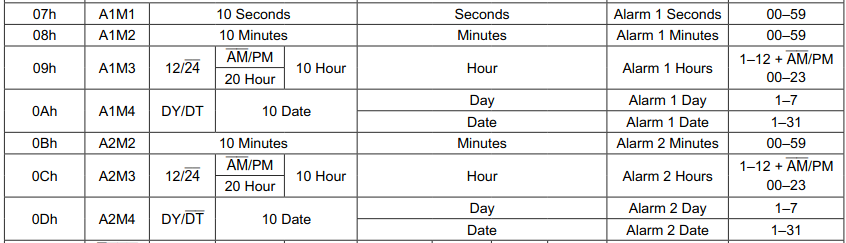
\includegraphics[width=0.8\textwidth]{images/alarmRegisters}
	\caption{Alarm 1 and Alarm 2 Registers}
	\label{fig:images-alarmRegister}
\end{figure}

\lstinputlisting[language=C++, caption={writeAlarm Function}]{snippets/writeAlarm.cpp}

The interrupt can be set by setting the $3^{rd}$ bit of the control register high.
This bit controls the square wave generator output, and, as such, setting the
bit high will disable the output when the interrupt alarm condition is met. The
``setInterrupt'' function takes two boolean inputs, which are used to confirm
setting the ``A1E'' and ``A2E'' alarm enable bits. If either boolean is true,
the interrupt bit is set high, along with the bit of the corresponding alarm. If
neither boolean is true, the interrupt bit is set low. Once all of the required
bits are set/cleared using the ``changeBits'' function, the value within the
buffer can be written to the register.

\begin{figure}[H]
	\centering
	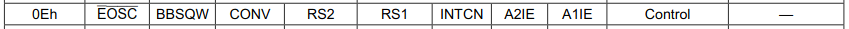
\includegraphics[width=0.8\textwidth]{images/controlRegister}
	\caption{Control Register}
	\label{fig:images-controlRegister}
\end{figure}

\lstinputlisting[language=C++, caption={set Interrupt Function}]{snippets/setInterrupt.cpp}
